\chapter{Test}
\section{Opgave 1}
\subsection{Opgave 1.2 speedup resultater}
\label{Speedup_Output}

\begin{figure}[h!]
\centering
\caption{Speedup output for input 10.000}
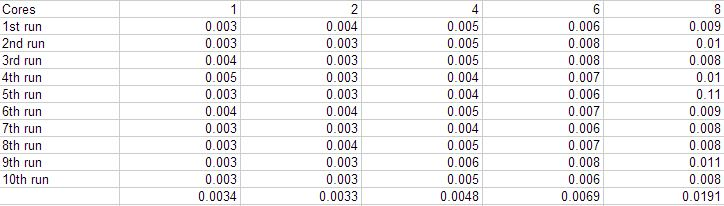
\includegraphics[width=\linewidth]{Images/oo2-1-2-SU10000}
\label{Speedup10.000}
\end{figure}

\begin{figure}[h!]
\centering
\caption{Speedup output for input 100.000}
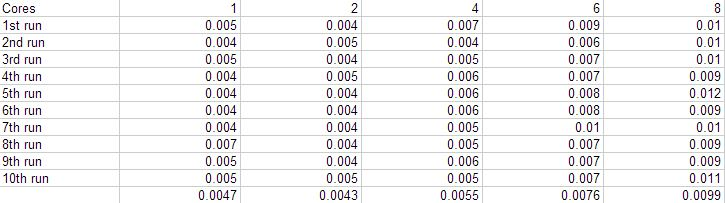
\includegraphics[width=\linewidth]{Images/oo2-1-2-SU100000}
\label{Speedup100.000}
\end{figure}

\begin{figure}[h!]
\centering
\caption{Speedup output for input 1.000.000}
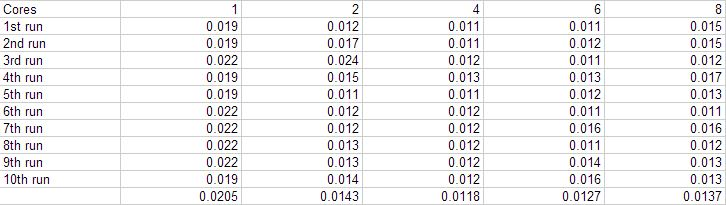
\includegraphics[width=\linewidth]{Images/oo2-1-2-SU1000000}
\label{Speedup1.000.000}
\end{figure}

\begin{figure}[h!]
\centering
\caption{Speedup output for input 10.000.000}
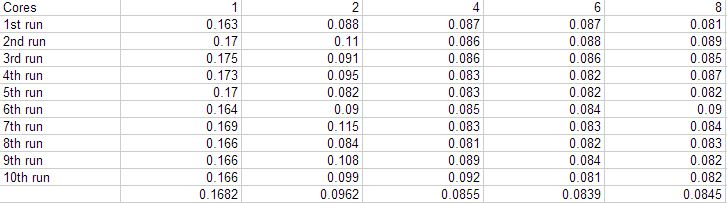
\includegraphics[width=\linewidth]{Images/oo2-1-2-SU10000000}
\label{Speedup10.000.000}
\end{figure}

\begin{figure}[h!]
\centering
\caption{Speedup output for input 100.000.000}
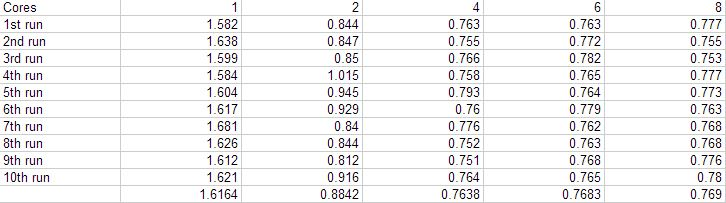
\includegraphics[width=\linewidth]{Images/oo2-1-2-SU100000000}
\label{Speedup100.000.000}
\end{figure}

\begin{figure}[h!]
\centering
\caption{Speedup output for input 50.000}
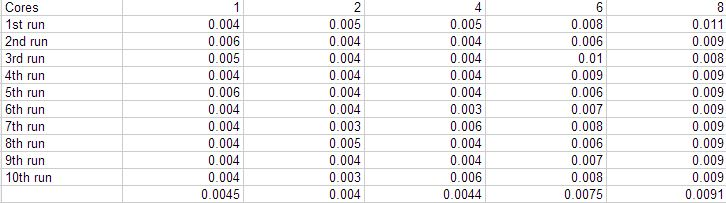
\includegraphics[width=\linewidth]{Images/oo2-1-2-SU50000}
\label{Speedup50.000}
\end{figure}

\begin{figure}[h!]
\centering
\caption{Speedup output for input 500.000}
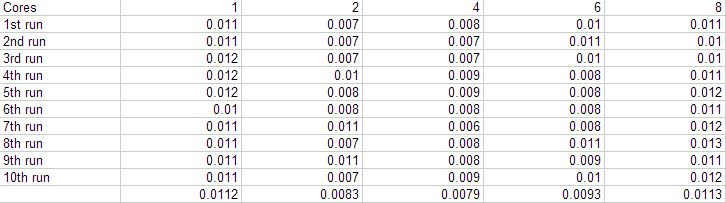
\includegraphics[width=\linewidth]{Images/oo2-1-2-SU500000}
\label{Speedup500.000}
\end{figure}

\begin{figure}[h!]
\centering
\caption{Speedup output for input 5.000.000}
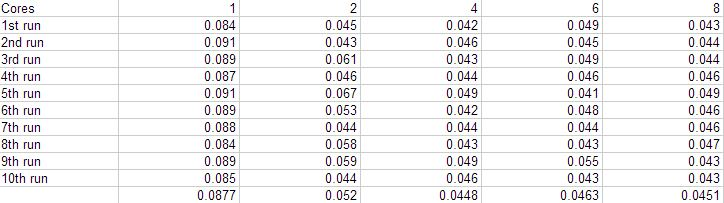
\includegraphics[width=\linewidth]{Images/oo2-1-2-SU5000000}
\label{Speedup5.000.000}
\end{figure}

\begin{figure}[h!]
\centering
\caption{Speedup output for input 50.000.000}
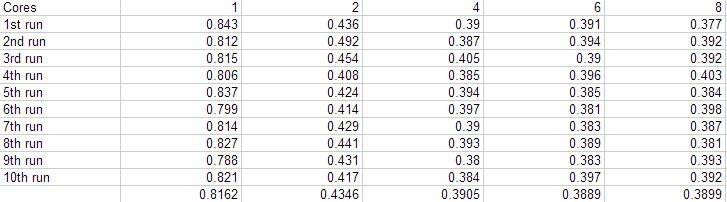
\includegraphics[width=\linewidth]{Images/oo2-1-2-SU50000000}
\label{Speedup50.000.000}
\end{figure}

\begin{figure}[h!]
\centering
\caption{Speedup output for input 500.000.000}
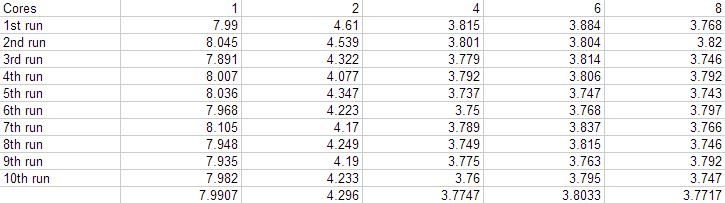
\includegraphics[width=\linewidth]{Images/oo2-1-2-SU500000000}
\label{Test3_1}
\end{figure}
\clearpage
\section{Opgave 3}
\subsection{Opgave 3 output}
\label{O3_Output}
./prodcons 5 3 3 10 15
\\Producer 1 produced ITEM\_0. Items in buffer: 1 (out of 10)
\\Producer 2 produced ITEM\_1. Items in buffer: 2 (out of 10)
\\Consumer 2 consumed ITEM\_0. Items in buffer: 1 (out of 10)
\\Consumer 1 consumed ITEM\_1. Items in buffer: 0 (out of 10)
\\Producer 0 produced ITEM\_2. Items in buffer: 1 (out of 10)
\\Consumer 0 consumed ITEM\_2. Items in buffer: 0 (out of 10)
\\Producer 1 produced ITEM\_3. Items in buffer: 1 (out of 10)
\\Consumer 2 consumed ITEM\_3. Items in buffer: 0 (out of 10)
\\Producer 0 produced ITEM\_4. Items in buffer: 1 (out of 10)
\\Consumer 0 consumed ITEM\_4. Items in buffer: 0 (out of 10)
\\Producer 0 produced ITEM\_5. Items in buffer: 1 (out of 10)
\\Consumer 1 consumed ITEM\_5. Items in buffer: 0 (out of 10)
\\Producer 1 produced ITEM\_6. Items in buffer: 1 (out of 10)
\\Producer 2 produced ITEM\_7. Items in buffer: 2 (out of 10)
\\Producer 0 produced ITEM\_8. Items in buffer: 3 (out of 10)
\\Consumer 2 consumed ITEM\_6. Items in buffer: 2 (out of 10)
\\Consumer 0 consumed ITEM\_7. Items in buffer: 1 (out of 10)
\\Consumer 1 consumed ITEM\_8. Items in buffer: 0 (out of 10)
\\Producer 1 produced ITEM\_9. Items in buffer: 1 (out of 10)
\\Consumer 0 consumed ITEM\_9. Items in buffer: 0 (out of 10)
\\Producer 1 produced ITEM\_10. Items in buffer: 1 (out of 10)
\\Consumer 0 consumed ITEM\_10. Items in buffer: 0 (out of 10)
\\Producer 2 produced ITEM\_11. Items in buffer: 1 (out of 10)
\\Producer 0 produced ITEM\_12. Items in buffer: 2 (out of 10)
\\Consumer 2 consumed ITEM\_11. Items in buffer: 1 (out of 10)
\\Consumer 1 consumed ITEM\_12. Items in buffer: 0 (out of 10)
\\Producer 0 produced ITEM\_13. Items in buffer: 1 (out of 10)
\\Producer 2 produced ITEM\_14. Items in buffer: 2 (out of 10)
\\Consumer 0 consumed ITEM\_13. Items in buffer: 1 (out of 10)
\\Consumer 1 consumed ITEM\_14. Items in buffer: 0 (out of 10)